\chapter{Marco Teórico}
\label{ch:marco}

% =====================================================================
% Sección 2.1 Trabajos Previos
% =====================================================================

\section{Trabajos previos}
\label{sec:trabajos_previos}
 
El antecedente directo de este proyecto es el trabajo desarrollado en la propia
Universidad de Sevilla sobre las mismas embarcaciones que se emplean aquí, por lo que
se describe en primer lugar y con mayor detalle. A continuación se resumen los
principales trabajos de la literatura sobre vehículos de superficie autónomos y
sistemas multi-USV.
 
% ---------------------------------------------------------------------
\subsection{Automatización de la plataforma Invader en la Universidad de Sevilla}
\label{subsec:trabajo_previo_invader}
 
Iniesta Fernández~\cite{iniesta2025} abordó en su Trabajo Fin de Máster la
automatización de una embarcación Invader Lipo 30000\,mAh, un barco cebador comercial
concebido para su manejo por radiocontrol. La embarcación dispone de un casco de tipo
catamarán de ABS de 5\,mm de espesor, con unas dimensiones de
$60 \times 40 \times 20$\,cm y un peso inferior a 5\,kg. Se impulsa mediante dos
motores MT 650 45T, cada uno con su propia hélice y su propio controlador electrónico
de velocidad (ESC) reversible, y se alimenta con dos baterías de litio de 7,4\,V y
15\,000\,mAh que proporcionan una autonomía declarada superior a tres horas. La
embarcación carece de timón: la dirección se obtiene exclusivamente mediante la
diferencia de velocidad entre ambos motores, lo que la convierte en un vehículo de
propulsión diferencial.
 
Como paso previo a la integración, el trabajo caracterizó mediante ingeniería inversa
la electrónica original. Los ESC reciben una señal PWM bidireccional de 50\,Hz, en la
que un ciclo de trabajo de entre el 7\,\% y el 8\,\% mantiene el motor en reposo,
valores superiores lo hacen avanzar (8,75\,\% en avance recto) y valores inferiores lo
hacen retroceder (6,25\,\% en retroceso). Los giros se obtienen aplicando ciclos de
trabajo distintos a cada motor. Esta caracterización definió la interfaz que el
autopiloto debía reproducir.
 
Sobre esta base se integró un autopiloto Pixhawk 6X, alimentado mediante un módulo de
potencia Holybro PM02D desde una batería independiente de 14,8\,V. El autopiloto se
configuró con el firmware ArduPilot Rover en su clase de chasis para barcos y se
gestionó desde la estación de control Mission Planner. El receptor de radiocontrol
original se conectó al autopiloto mediante el protocolo SBUS, y las salidas se
configuraron como acelerador izquierdo y derecho, correspondientes al esquema de
dirección diferencial. La principal dificultad técnica fue la frecuencia de la señal
de salida: el tipo de salida previsto en ArduPilot para motores de escobillas
bipolares genera una PWM de 20\,kHz, pensada para gobernar directamente un puente H,
mientras que los ESC de la embarcación esperan una señal de tipo servo de 50\,Hz. El
problema se resolvió seleccionando el tipo de salida estándar, reasignando los canales
del receptor y recalibrando sus rangos, de modo que el autopiloto reprodujera las
señales generadas por el mando original. Además, se configuró el canal 5 de la emisora
como conmutador entre los modos \textit{Manual} y \textit{Auto}, lo que permite al
operador recuperar el control en cualquier momento.
 
Para la telemetría se instalaron radiomódems RFD900X en la banda de 900\,MHz,
conectados al puerto TELEM1 del autopiloto y configurados con el mismo canal en ambos
extremos. Las pruebas de alcance fueron de carácter cualitativo: se comprobó que la
telemetría seguía recibiéndose en la estación de control a distancias crecientes,
aunque se observó una respuesta más lenta en los límites del alcance. Para poder armar
el vehículo se desactivaron las comprobaciones previas al armado del autopiloto.
Finalmente, se planificaron rutas de waypoints en Mission Planner y se realizaron
pruebas en exterior, en las que se verificó con osciloscopio la conmutación entre
modos y la frecuencia de las señales, y se constató que la embarcación seguía de forma
autónoma los waypoints definidos. La validación fue de carácter funcional, sin registro
de métricas cuantitativas de error de trayectoria, alcance o latencia.
 
Como desarrollo futuro, el trabajo propone incorporar un ordenador a bordo con ROS~2
que defina los movimientos de forma autónoma, en lugar de depender de rutas fijadas
manualmente desde la estación de control; utilizar varias embarcaciones de forma
simultánea en misiones coordinadas; y añadir sensores de calidad del agua, ya sea
practicando aperturas en el casco o mediante una boya remolcada.
 
En conjunto, el trabajo dejó una embarcación Invader con autopiloto configurado, enlace
de telemetría y navegación por waypoints validada de forma funcional, operando como
vehículo individual y sin ordenador a bordo. La extensión a varias embarcaciones
coordinadas mediante ROS~2 quedó planteada como línea de trabajo futuro.
 
% ---------------------------------------------------------------------
\subsection{Sistemas USV y multi-USV en la literatura}
\label{subsec:literatura_usv}
 
La revisión de Dunbabin y Marques~\cite{dunbabin2012} identifica los sistemas marinos
como los más maduros de la robótica ambiental y señala como retos abiertos la
coordinación cooperativa con bajo ancho de banda y latencias asíncronas, así como la
fiabilidad de las plataformas en campo. Los trabajos más cercanos a este proyecto pueden
agruparse en dos líneas.
 
\newpage

En primer lugar, los trabajos centrados en la cooperación entre varios vehículos de
superficie:
 
\begin{itemize}
  \item Manjanna \textit{et al.}~\cite{manjanna2018} emplean dos ASV con roles
    diferenciados: uno construye un mapa de clorofila mediante procesos gaussianos y el
    otro selecciona los puntos de muestreo físico. El sistema se valida en un embalse
    real, aunque sin modelar la pérdida de comunicación entre vehículos.
  \item Wen \textit{et al.}~\cite{wen2022} resuelven la navegación y la asignación de
    áreas de una flota de dos a cuatro USV mediante el algoritmo MADDPG, con una
    validación limitada a simulación.
  \item Singh \textit{et al.}~\cite{singh2020} coordinan flotas de tres y cuatro USV
    mediante una ruta planificada con A* y un objetivo virtual en el marco de
    Serret--Frenet, también validado únicamente en simulación.
\end{itemize}
 
En segundo lugar, los trabajos que desarrollan y validan en campo plataformas USV de
bajo coste, todos ellos con una arquitectura de doble controlador formada por un
autopiloto para el control de bajo nivel y un ordenador a bordo para las tareas de alto
nivel:
 
\begin{itemize}
  \item Gogendeau \textit{et al.}~\cite{gogendeau2024} construyen un ASV de código
    abierto con Pixhawk, ArduPilot Rover y Raspberry Pi, comunicado mediante RFD900x a
    868\,MHz, y reportan su vuelco con vientos superiores a 20 nudos.
  \item Sotelo-Torres \textit{et al.}~\cite{sotelo2023} integran Pixhawk, Raspberry Pi 4
    y telemetría RFD900+, con errores de seguimiento de hasta 2,5\,m en los giros.
  \item Kumar \textit{et al.}~\cite{kumar2025} desarrollan dos USV de hardware idéntico
    con ArduPilot, Jetson Orin Nano y ROS~2 Humble, empleados de forma secuencial, y
    documentan las dificultades de los controladores nativos de ArduPilot para mantener
    el rumbo bajo corrientes intensas.
  \item Sears \textit{et al.}~\cite{sears2024} integran un USV comercial con ROS~2 sobre
    una Jetson AGX Orin y reportan un alcance del enlace WiFi de entre 0,5 y 1\,km.
  \item Mamani \textit{et al.}~\cite{Cite9} implementan un USV para muestreo de agua
    con ROS~2, Nav2, posicionamiento GNSS RTK y supervisión mediante LoRa a 915\,MHz.
\end{itemize}
 
En conjunto, la cooperación entre varios USV se ha validado mayoritariamente en
simulación o sobre plataformas de investigación dedicadas, mientras que los trabajos
que emplean hardware de bajo coste basado en ArduPilot y se validan en campo se centran
en un único vehículo.

% =====================================================================
% Sección 2.2 Conceptos clave
% =====================================================================

\section{Conceptos clave}
\label{sec:conceptos}

A continuación se definen los conceptos empleados a lo largo del informe que, sin ser
elementales, resultan necesarios para comprender el diseño, la integración y la
validación del sistema desarrollado. Los conceptos asociados a modelos o ecuaciones
específicos, como los grados de libertad del vehículo, el error de seguimiento de
trayectoria o las métricas de los enlaces de comunicación, se definen en la sección
correspondiente de este capítulo.
 
\begin{description}
 
  \item[Vehículo de superficie no tripulado (USV):] embarcación que opera sobre la
    superficie del agua sin tripulación a bordo, ya sea teleoperada desde una estación
    remota o con capacidad de navegación autónoma. Desde el punto de
    vista del control, se trata de un vehículo no holonómico y habitualmente
    subactuado, es decir, con menos actuadores independientes que grados de libertad,
    cuyo movimiento se ve afectado por perturbaciones ambientales como el viento, el
    oleaje y las corrientes~\cite{kumar2025} \cite{jin2025}. En la literatura también se les
    denomina vehículos de superficie autónomos (ASV) o Unmanned Surface Vehicles (USV).
 
  \item[Sistema multi-USV cooperativo:] conjunto de dos o más USV que operan de forma
    simultánea en un mismo entorno y comparten información para cumplir un objetivo
    común. Frente a un único vehículo, la cooperación permite cubrir mayores áreas en
    menos tiempo, repartir tareas entre vehículos y aportar redundancia frente al fallo
    de uno de ellos, a costa de requerir mecanismos de comunicación y coordinación entre
    los vehículos~\cite{dunbabin2012}.
 
  \item[Autopiloto:] controlador embebido que ejecuta, sobre un sistema operativo de
    tiempo real, las tareas de bajo nivel de un vehículo no tripulado: la lectura de sus
    sensores inerciales y de posicionamiento, la estimación de su estado, el cálculo de
    las consignas de rumbo y velocidad y la generación de las señales que gobiernan los
    actuadores. En investigación predominan los autopilotos de hardware abierto, que
    ejecutan firmware de código abierto configurable para distintos tipos de vehículo,
    incluidas las embarcaciones~\cite{aliane2026}.
  
  \item[Posicionamiento GNSS y RTK:] los sistemas globales de navegación por satélite
    (GNSS), como GPS, Galileo o GLONASS, determinan la posición del receptor a partir de
    las señales de una constelación de satélites, con errores típicos de varios metros.
    La técnica RTK (\textit{Real-Time Kinematic}) mejora esa precisión aplicando en
    tiempo real las correcciones calculadas por una estación de referencia de posición
    conocida, lo que reduce el error hasta el orden de centímetros~\cite{Cite13}.
 
  \item[Estimación de estado:] proceso mediante el cual un sistema de navegación
    obtiene la posición, la velocidad y la orientación del vehículo a partir de medidas
    de sensores que, por separado, son ruidosas o incompletas. Los autopilotos
    actuales fusionan las medidas de giróscopos, acelerómetros, magnetómetro, barómetro
    y receptor GNSS mediante un filtro de Kalman extendido (EKF), que estima los estados
    no medibles directamente, como la posición y la velocidad, y filtra el ruido de los
    sensores para refinar la orientación~\cite{aliane2026}.
 
  \item[Armado y comprobaciones previas al armado:] el armado es la acción que habilita
    la salida de potencia hacia los propulsores de un vehículo; mientras está
    desarmado, los motores no responden a ninguna consigna. Antes de permitir el armado,
    el autopiloto ejecuta un conjunto de comprobaciones de seguridad que verifican, por
    ejemplo, la validez de las lecturas del receptor GNSS y del compás, y bloquea el
    armado si detecta algún problema~\cite{iniesta2025} \cite{kumar2025}.
 
  \item[Ordenador a bordo:] procesador de propósito general (\textit{companion
    computer}) instalado junto al autopiloto y conectado a este mediante un enlace
    serie o Ethernet. Recibe la telemetría del autopiloto y ejecuta las tareas de alto
    nivel que exceden su capacidad, como el procesamiento de imágenes, la planificación
    de trayectorias, el registro de datos o la coordinación con otros vehículos. Suele
    tratarse de placas compactas basadas en arquitectura ARM con sistema operativo
    Linux; las de mayor capacidad incorporan además un procesador gráfico (GPU) que
    acelera las tareas de visión y de aprendizaje automático~\cite{kumar2025} \cite{aliane2026}.
 
  \item[Estación de control en tierra (GCS):] equipo y aplicación desde los cuales el
    operador configura el vehículo, planifica las misiones, supervisa su estado en
    tiempo real y envía comandos durante la operación. Habitualmente permite también
    cargar el firmware del autopiloto y ajustar sus parámetros~\cite{iniesta2025} \cite{aliane2026}.
 
  \item[Telemetría:] intercambio continuo, a través de un enlace inalámbrico, de la
    información de estado del vehículo, como la posición, el rumbo, la velocidad, el
    modo de operación o el nivel de batería, hacia la estación de control, junto con los
    comandos enviados en sentido inverso. Este intercambio permite supervisar el
    vehículo, modificar sus parámetros o su misión durante la operación y recuperar su
    control ante una anomalía~\cite{iniesta2025} \cite{aliane2026}.
 
\end{description}
 

% =====================================================================
% Sección 2.3 Modelo del vehículo de superficie con propulsión diferencial
% =====================================================================
 
\section{Modelo y guiado del vehículo de superficie}
\label{sec:modelo_usv}
 
% ---------------------------------------------------------------------
\subsection{Modelo de un vehículo con propulsión diferencial}
\label{subsec:modelo_propulsion}
 
El movimiento de un vehículo marino se describe mediante dos marcos de
referencia~\cite{jin2025}: un marco inercial local de tipo NED
(\textit{North--East--Down}), fijo a la superficie terrestre, y un marco solidario al
vehículo, con el eje $x$ hacia la proa, el eje $y$ hacia estribor y el eje $z$ hacia
abajo (Figura~\ref{fig:marcos_usv}). Como cualquier cuerpo rígido, una embarcación
tiene seis grados de libertad: tres traslaciones a lo largo de los ejes del cuerpo,
denominadas avance (eje $x$), deriva (eje $y$) y arfada (eje $z$, movimiento vertical
de subida y bajada), y tres rotaciones alrededor de esos mismos ejes, denominadas
balanceo, cabeceo y guiñada~\cite{jin2025}. En un vehículo de superficie, la arfada,
el balanceo y el cabeceo están sometidos a fuerzas restauradoras de flotación que
devuelven la embarcación a su posición de equilibrio, por lo que, a baja velocidad y en
aguas tranquilas, se reducen a pequeñas oscilaciones que no afectan a la trayectoria.
Además, los propulsores solo actúan en el plano horizontal. Por ello, el movimiento
relevante para la navegación se describe en ese plano con tres grados de libertad:
avance, deriva y guiñada~\cite{jin2025}. La posición y el rumbo del vehículo en el marco
inercial, $\boldsymbol{\eta}$, y sus velocidades en el marco del cuerpo,
$\boldsymbol{\nu}$, se relacionan mediante
\begin{equation}
  \dot{\boldsymbol{\eta}} = \mathbf{R}(\psi)\,\boldsymbol{\nu},
  \qquad
  \boldsymbol{\eta} = \begin{bmatrix} x \\ y \\ \psi \end{bmatrix},
  \quad
  \boldsymbol{\nu} = \begin{bmatrix} u \\ v \\ r \end{bmatrix},
  \quad
  \mathbf{R}(\psi) =
  \begin{bmatrix}
    \cos\psi & -\sin\psi & 0 \\
    \sin\psi &  \cos\psi & 0 \\
    0 & 0 & 1
  \end{bmatrix}
  \label{eq:cinematica}
\end{equation}
donde $x$ e $y$ son las coordenadas norte y este, $\psi$ es el rumbo, $u$ y $v$ son las
velocidades de avance y de deriva, y $r$ es la velocidad angular de guiñada. Una
velocidad de deriva no nula, provocada por el viento o las corrientes, desplaza al
vehículo lateralmente respecto a su rumbo.
 
\begin{figure}[htbp]
  \centering
  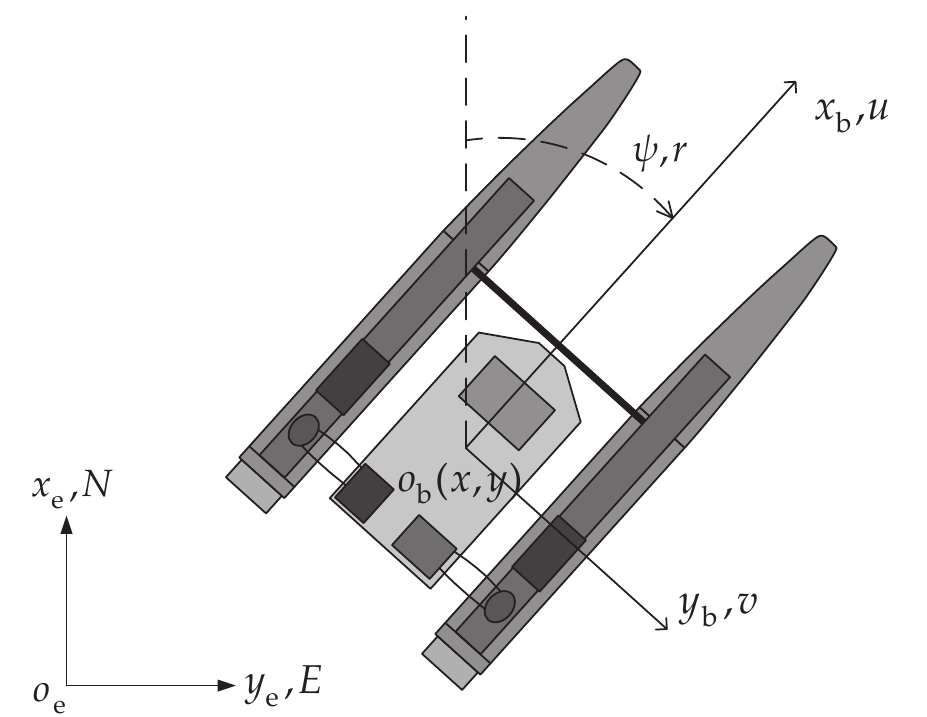
\includegraphics[width=0.55\textwidth]{fig/fig_marcos_usv_jin2025.png}
  \caption{Marco de referencia inercial y marco del cuerpo de un USV de tipo
    catamarán~\cite{jin2025}.}
  \label{fig:marcos_usv}
\end{figure}
 
La dinámica en el plano horizontal se expresa mediante el modelo vectorial de
tres grados de libertad~\cite{jin2025}:
\begin{equation}
  \mathbf{M}\,\dot{\boldsymbol{\nu}} + \mathbf{C}(\boldsymbol{\nu})\,\boldsymbol{\nu}
  + \mathbf{D}(\boldsymbol{\nu})\,\boldsymbol{\nu} = \boldsymbol{\tau}
  \label{eq:fossen}
\end{equation}
donde $\mathbf{M}$ es la matriz de masa e inercia, que incluye la masa añadida del agua
que el casco arrastra al acelerar; $\mathbf{C}(\boldsymbol{\nu})$ agrupa los efectos
centrípetos y de Coriolis; $\mathbf{D}(\boldsymbol{\nu})$ representa el amortiguamiento
hidrodinámico; y $\boldsymbol{\tau}$ es el vector de fuerzas y momento de los
propulsores. En un vehículo sin timón con dos propulsores paralelos separados una
distancia $2d$, este vector resulta~\cite{kumar2025}
\begin{equation}
  \boldsymbol{\tau} =
  \begin{bmatrix} T_1 + T_2 & 0 & (T_1 - T_2)\,d \end{bmatrix}^{T}
  \label{eq:tau}
\end{equation}
donde $T_1$ y $T_2$ son los empujes de babor y de estribor. La suma de ambos produce el
avance y su diferencia genera el momento de guiñada. Al no existir ningún actuador que
genere fuerza en deriva, el vehículo es subactuado~\cite{kumar2025}, y su deriva
solo puede corregirse de forma indirecta modificando el rumbo. En la práctica, el
autopiloto no calcula los empujes a partir del modelo, sino que combina una consigna de
avance y una de giro para obtener la orden de cada motor, configuración conocida como
dirección diferencial o \textit{skid steering}~\cite{kumar2025, iniesta2025}.
 
Por otra parte, la estabilidad transversal de una embarcación ante la incorporación de
carga se evalúa mediante la altura metacéntrica $GM$, distancia entre el centro de
gravedad $G$ y el metacentro transversal $M$, punto en torno al cual oscila el empuje de
flotación cuando la embarcación se inclina ligeramente~\cite{biran2014}:
\begin{equation}
  GM = KB + \frac{I_T}{\nabla} - KG,
  \qquad
  KG = \frac{m_0\,KG_0 + \sum_{j} m_j\,z_j}{m_0 + \sum_{j} m_j}
  \label{eq:gm}
\end{equation}
donde $K$ es la quilla, $KB$ la altura del centro de carena, $I_T$ el momento de
inercia transversal del área de flotación, $\nabla$ el volumen desplazado y $KG$ la
altura del centro de gravedad, que se recalcula a partir de la embarcación vacía
($m_0$, $KG_0$) y de la masa $m_j$ y altura $z_j$ de cada componente añadido. La
embarcación es estable si $GM > 0$; en los cascos de tipo catamarán, la separación entre
cascos aumenta notablemente $I_T$ y, con ello, la estabilidad~\cite{biran2014}.
 
% ---------------------------------------------------------------------
\subsection{Guiado por waypoints y error de seguimiento}
\label{subsec:guiado_waypoints}
 
En la navegación autónoma, la misión se define como una secuencia de waypoints cuyas
coordenadas geográficas se convierten a coordenadas locales en el marco NED, de modo que
la trayectoria deseada queda formada por segmentos rectos. El vehículo conmuta al
segmento siguiente cuando entra en un círculo de radio predefinido alrededor del
waypoint objetivo, denominado círculo de aceptación~\cite{jin2025}. La desviación
respecto al segmento activo se cuantifica mediante el error transversal $y_{e}^{p}$,
distancia perpendicular entre el vehículo y la recta que une los waypoints
$(x_{i}^{n}, y_{i}^{n})$ y $(x_{i+1}^{n}, y_{i+1}^{n})$
(Figura~\ref{fig:error_transversal}), que puede obtenerse
geométricamente proyectando la posición del vehículo sobre la normal al
segmento~\cite{jin2025}:
\begin{equation}
  y_{e}^{p} = -\left(x^{n} - x_{i}^{n}\right)\sin\pi_{p}
              + \left(y^{n} - y_{i}^{n}\right)\cos\pi_{p}
  \label{eq:error_transversal}
\end{equation}
donde $(x^{n}, y^{n})$ es la posición del vehículo y $\pi_{p}$ el ángulo del segmento
respecto al norte. La ley de guiado por línea de vista (LOS, \textit{Line of Sight})
reduce este error orientando el vehículo hacia un punto situado a una distancia de
anticipación $\Delta$ por delante de su proyección sobre el segmento~\cite{jin2025}:
\begin{equation}
  \psi_{d} = \pi_{p} - \arctan\!\left(\frac{y_{e}^{p}}{\Delta}\right)
  \label{eq:los}
\end{equation}
Un valor pequeño de $\Delta$ acelera la convergencia a costa de oscilaciones, y la
variante integral (ILOS) añade la integral del error para compensar perturbaciones
persistentes como el viento o las corrientes~\cite{jin2025}.
 
\begin{figure}[htbp]
  \centering
  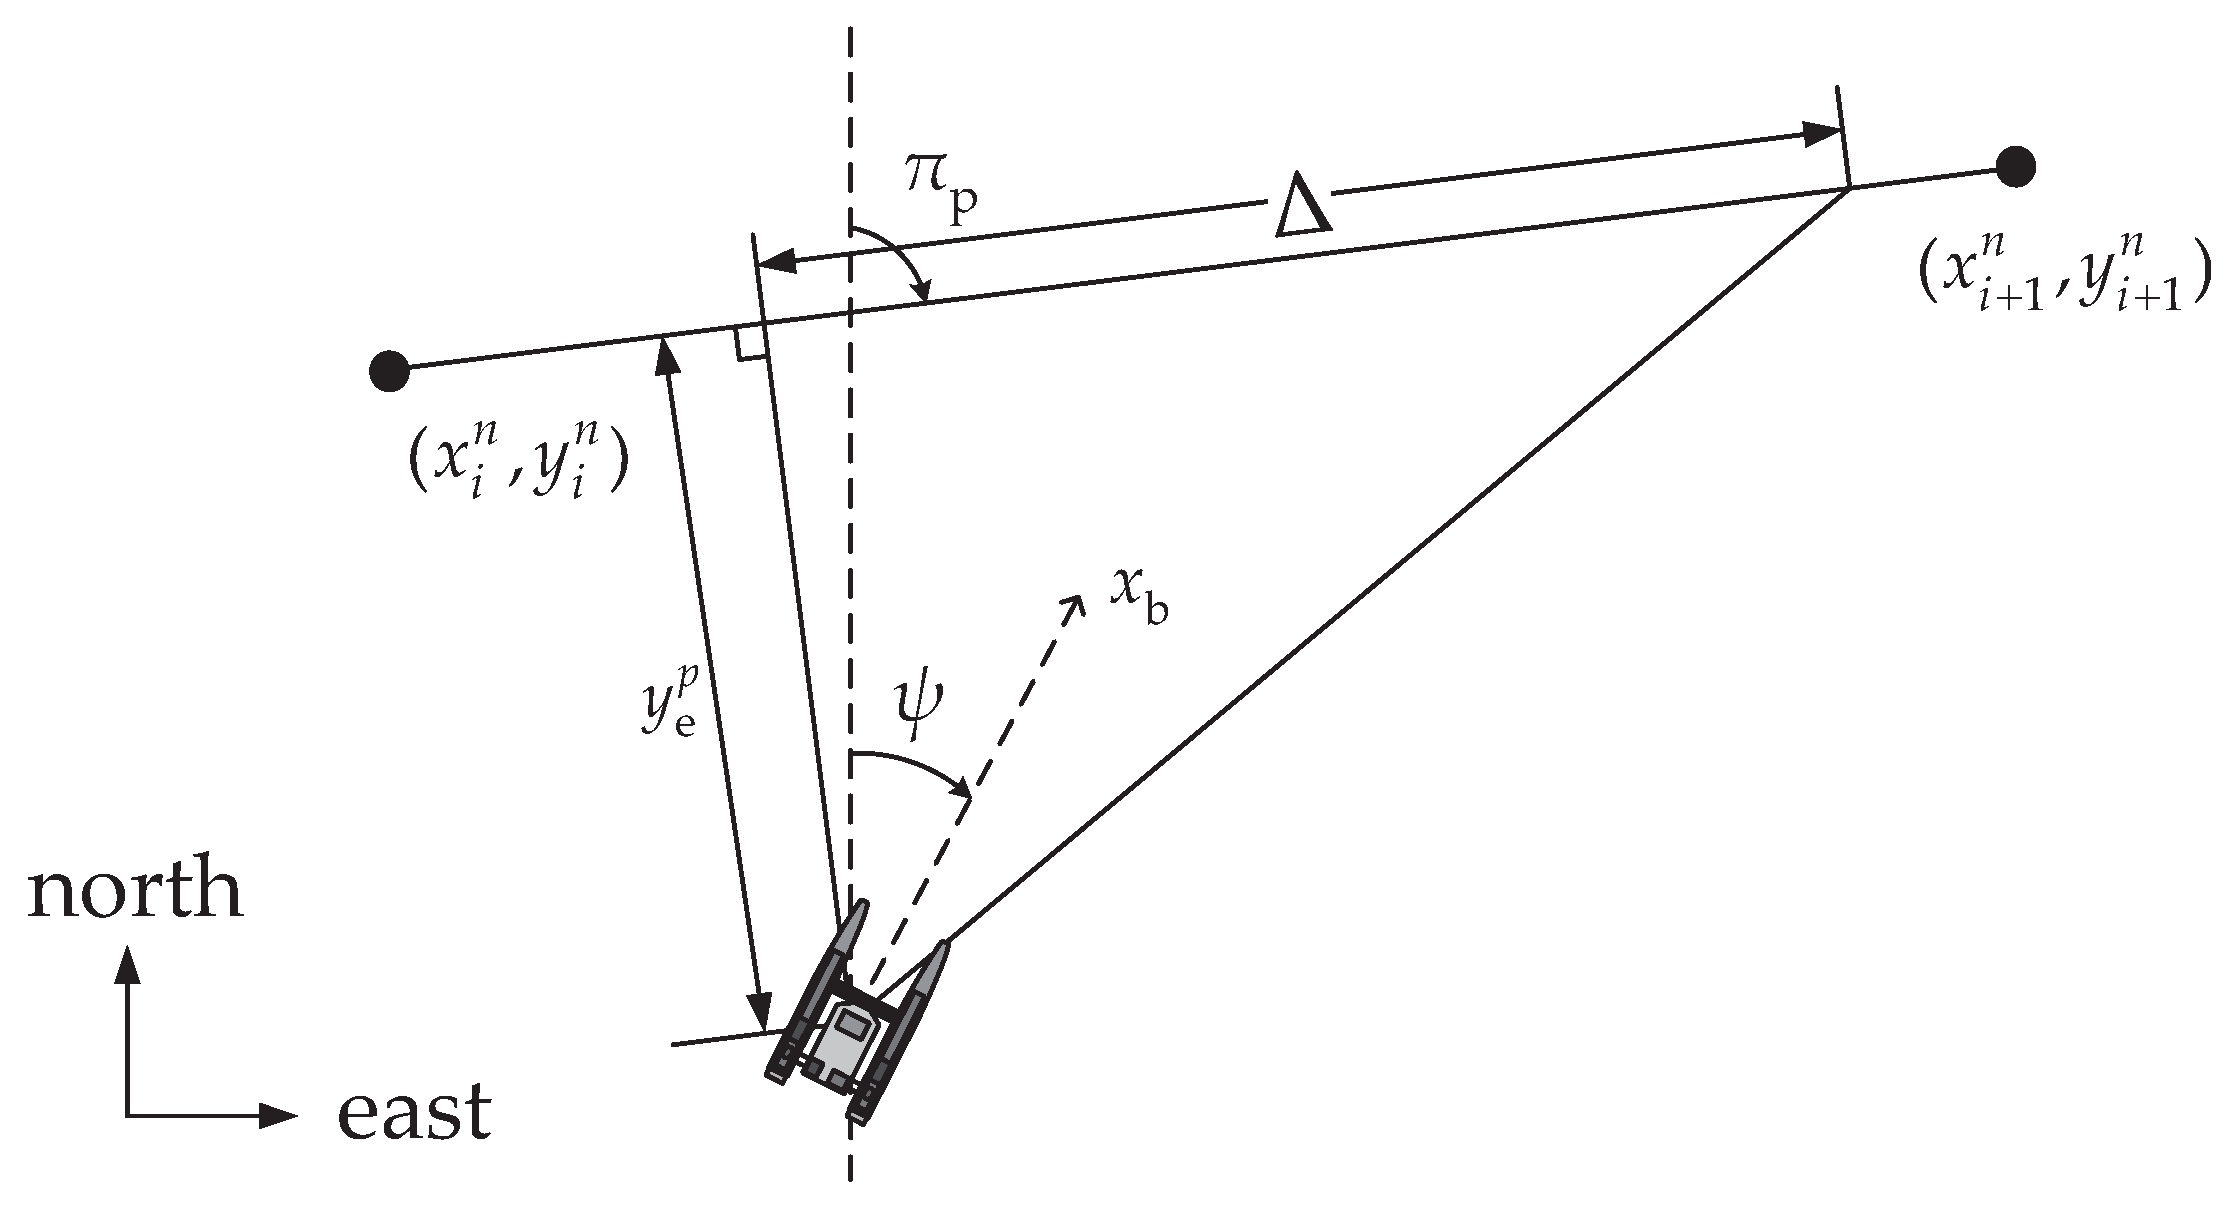
\includegraphics[width=0.65\textwidth]{fig/fig_marcos_usv_jin2025_2.png}
  \caption{Geometría del guiado por línea de vista: error transversal $y_{e}^{p}$,
    ángulo del segmento $\pi_{p}$, distancia de anticipación $\Delta$ y rumbo $\psi$ ~\cite{jin2025}.}
  \label{fig:error_transversal}
\end{figure}
 
En los autopilotos comerciales, un controlador de guiado calcula el rumbo necesario para
converger al waypoint y lo entrega a un lazo interno de rumbo, que actúa sobre el empuje
diferencial de los propulsores, mientras otro lazo regula la velocidad de
avance~\cite{kumar2025}. La precisión de seguimiento a lo largo
de una misión se resume habitualmente mediante la raíz del error cuadrático medio del
error transversal,
$\mathrm{RMSE} = \sqrt{\tfrac{1}{N}\sum_{k=1}^{N}\bigl(y_{e,k}^{p}\bigr)^{2}}$, junto
con el error máximo, que suele concentrarse en los giros~\cite{sotelo2023}.
 

% =====================================================================
% Sección 2.4 Arquitectura de software: ROS 2 y su integración con el autopiloto
% Requiere: graphicx
% =====================================================================
 
\section{Arquitectura de software: ROS~2 y su integración con el autopiloto}
\label{sec:arquitectura_software}
 
% ---------------------------------------------------------------------
\subsection{Elementos de ROS~2}
\label{subsec:elementos_ros2}
 
ROS~2 (\textit{Robot Operating System 2}) es un \textit{middleware} de código abierto
que estructura el software de un robot en procesos independientes y modulares,
denominados nodos, cada uno responsable de una única función, como leer un sensor,
calcular una trayectoria o gobernar un actuador~\cite{roach2023} \cite{albatati2026}. Los
nodos se comunican mediante cuatro mecanismos:
 
\begin{itemize}
  \item \textbf{Tópicos:} canales con nombre por los que circulan mensajes de un tipo
    definido. Un nodo publicador envía mensajes a un tópico y cualquier número de nodos
    suscriptores los reciben, sin que emisor y receptor necesiten conocerse
    (Figura~\ref{fig:ros2_elementos}a). Es el mecanismo adecuado para flujos continuos
    de datos, como la posición o el estado de un vehículo~\cite{roach2023}.
  \item \textbf{Servicios:} interacciones de petición y respuesta entre un nodo cliente
    y un nodo servidor, empleadas para operaciones puntuales, como consultar un dato o
    cambiar una configuración~\cite{roach2023}.
  \item \textbf{Acciones:} tareas de larga duración en las que un cliente envía un
    objetivo, el servidor informa periódicamente del progreso y, al terminar, devuelve
    un resultado (Figura~\ref{fig:ros2_elementos}b). Son adecuadas, por ejemplo, para
    desplazar un robot hasta una posición objetivo~\cite{roach2023}.
  \item \textbf{Parámetros:} valores de configuración propios de cada nodo, que pueden
    consultarse y modificarse sin recompilar el código~\cite{albatati2026}.
\end{itemize}
 
\begin{figure}[htbp]
  \centering
  \begin{minipage}[b]{0.48\textwidth}
    \centering
    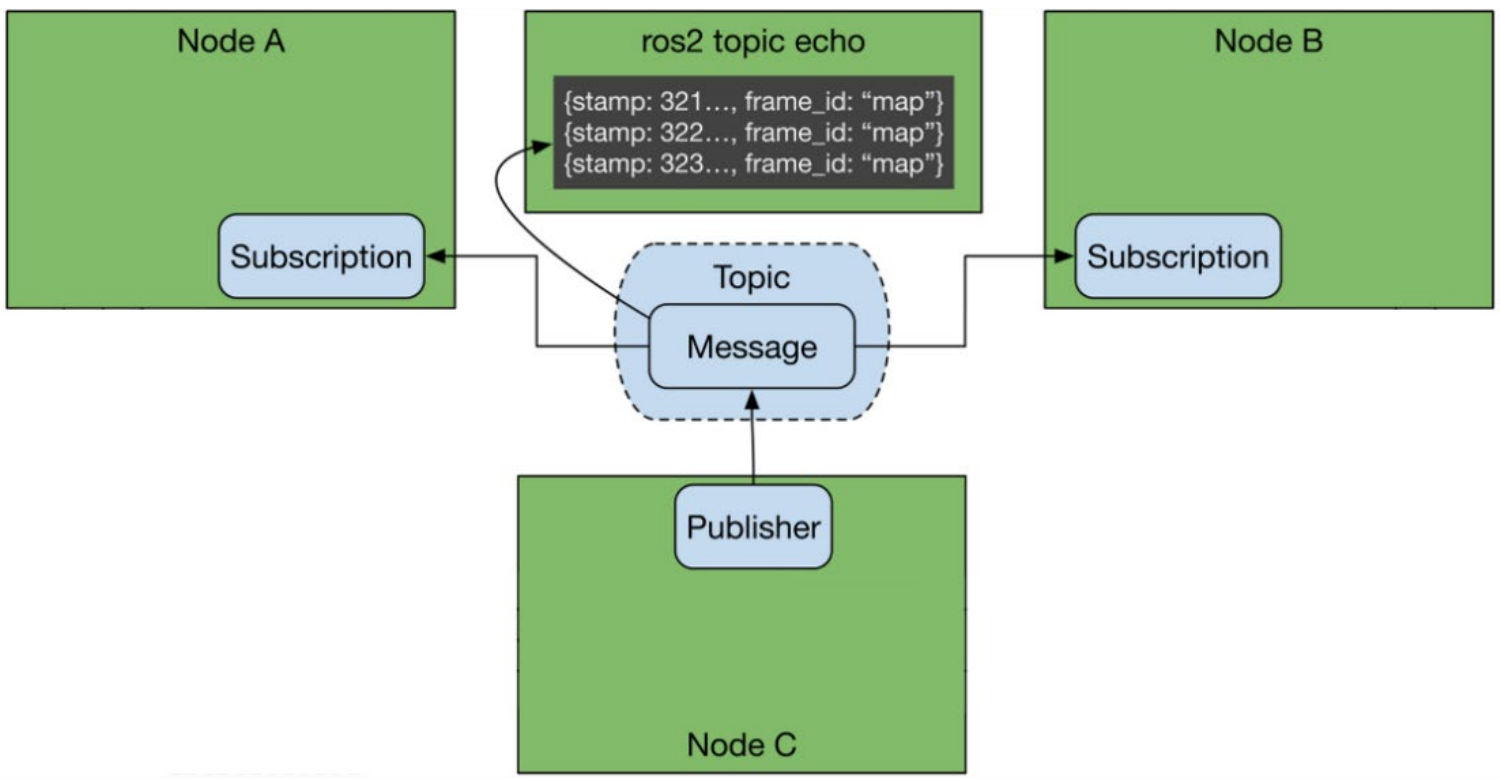
\includegraphics[width=\textwidth]{fig/fig_ros2_topicos_roach2023.png}\\[2pt]
    \small (a) Tópicos: publicación y suscripción.
  \end{minipage}
  \hfill
  \begin{minipage}[b]{0.48\textwidth}
    \centering
    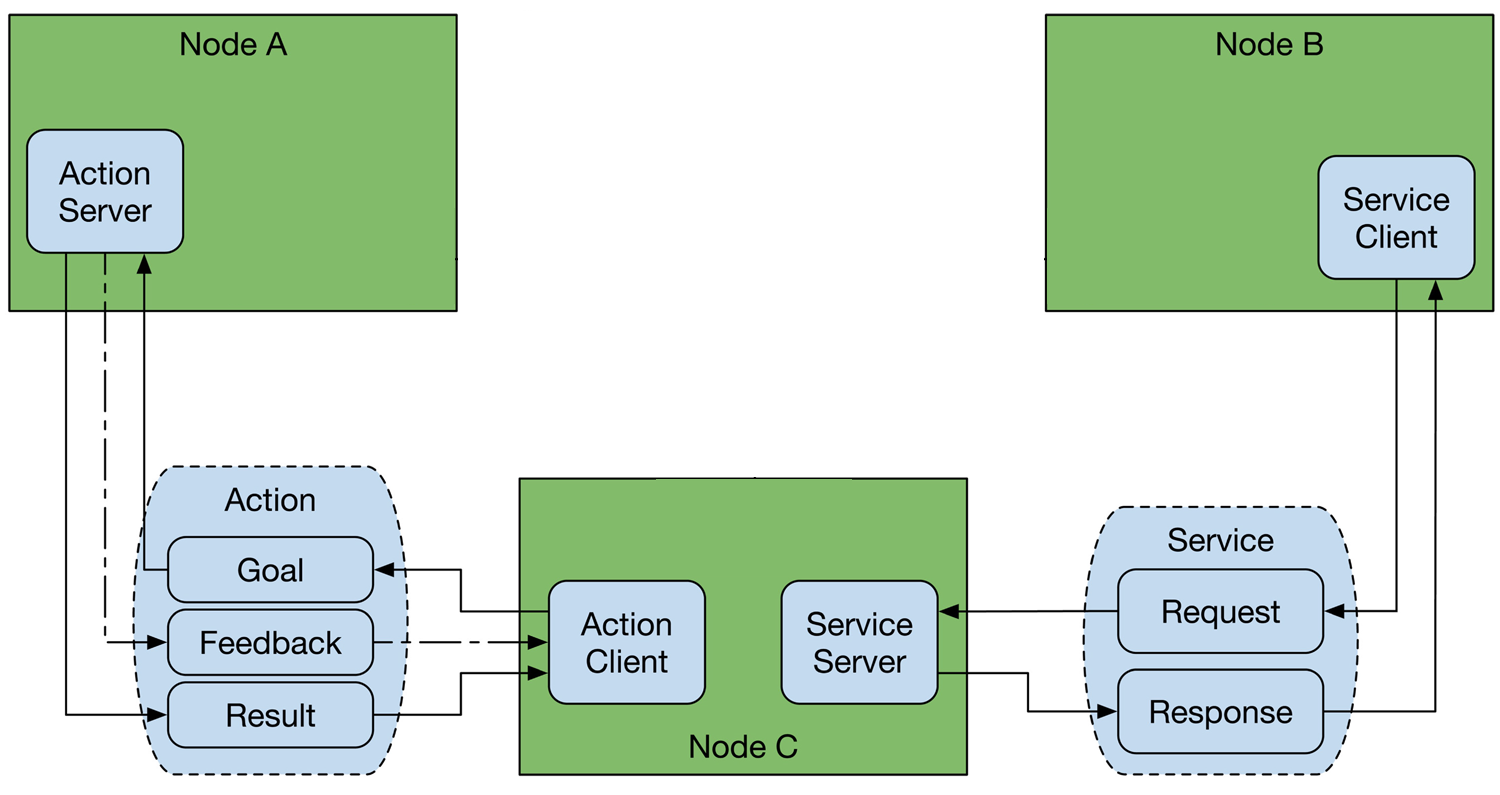
\includegraphics[width=\textwidth]{fig/fig_ros2_servicios_acciones_roach2023.png}\\[2pt]
    \small (b) Servicios y acciones.
  \end{minipage}
  \caption{Mecanismos de comunicación entre nodos en ROS~2 ~\cite{roach2023}.}
  \label{fig:ros2_elementos}
\end{figure}

Cada mensaje publicado en un tópico puede incluir una cabecera con la marca de tiempo
del instante en que se generó el dato, como se aprecia en los mensajes de la
Figura~\ref{fig:ros2_elementos}a~\cite{roach2023}. Comparando esa marca con el instante
en que el mensaje llega al nodo suscriptor se obtiene la latencia del dato, que en ROS~2
resulta de la suma del retardo de comunicación y del tiempo de procesamiento del
\textit{middleware}~\cite{albatati2026}.
 
 
% ---------------------------------------------------------------------
\subsection{Middleware DDS y calidad de servicio}
\label{subsec:dds_qos}
 
A diferencia de ROS~1, que dependía de un nodo maestro central para registrar a los
nodos, ROS~2 se apoya en DDS (\textit{Data Distribution Service}), un estándar de
comunicación que descubre a los nodos de forma descentralizada y elimina ese punto
único de fallo, de modo que nodos ejecutados en equipos distintos de una misma red se
comunican directamente entre sí~\cite{albatati2026}. DDS ofrece además políticas de
calidad de servicio (QoS) configurables para cada tópico. La más relevante es la
fiabilidad: el modo \textit{reliable} retransmite los mensajes perdidos, mientras que el
modo \textit{best effort} los descarta en favor de una menor latencia. En la práctica,
el modo \textit{reliable} añade entre 1 y 10\,ms de latencia, pero reduce la pérdida de
paquetes hasta en un 40\,\%, y el tamaño del historial de mensajes almacenados permite
equilibrar la variación de la latencia frente al retardo máximo~\cite{albatati2026}.
 
En sistemas con varios robots, ROS~2 no requiere un nodo central: los dominios DDS
permiten separar redes lógicas, y los espacios de nombres (\textit{namespaces}) y la
reasignación de tópicos aíslan el tráfico de cada robot dentro de una misma red,
manteniendo la comunicación selectiva entre ellos~\cite{albatati2026}. Así, por ejemplo,
dos vehículos pueden ejecutar los mismos nodos publicando en tópicos diferenciados por
el prefijo de su espacio de nombres.
 
% ---------------------------------------------------------------------
\subsection{Integración con el autopiloto: MAVLink y MAVROS}
\label{subsec:mavros}
 
El firmware de un autopiloto organiza el comportamiento del vehículo en modos de
operación, que determinan quién lo gobierna y con qué referencia. Los más habituales en
vehículos de superficie son los siguientes: en el modo \textit{Manual}, el operador controla directamente los propulsores
desde la emisora de radiocontrol~\cite{iniesta2025}; en \textit{Auto}, el vehículo
ejecuta una ruta de waypoints previamente cargada; en \textit{Guided}, acepta consignas
de velocidad, rumbo o posición enviadas en tiempo real por un sistema externo, como un
ordenador a bordo; en \textit{Loiter}, mantiene su posición y rumbo frente a la
corriente o el viento; y en \textit{RTL}, regresa de forma autónoma al punto de partida,
por ejemplo ante una batería baja~\cite{kumar2025}.
 
La comunicación entre el autopiloto, la estación de control y el ordenador a bordo se
realiza mediante MAVLink (\textit{Micro Air Vehicle Link}), un protocolo ligero de
mensajes binarios, de entre 12 y 280 bytes en su versión 2.0, que puede transmitirse
tanto por enlaces serie de radio como por redes IP. MAVLink permite además enrutar
mensajes entre varios sistemas y componentes, cada uno con un identificador único, de
modo que varios vehículos pueden compartir una misma red y una misma estación de
control~\cite{aliane2026}.
 
La conexión entre ROS~2 y el autopiloto se realiza mediante MAVROS, un paquete que actúa
como puente: traduce los mensajes MAVLink del autopiloto en tópicos y servicios de
ROS~2 y, en sentido inverso, convierte en mensajes MAVLink las consignas publicadas por
los nodos~\cite{aliane2026}. La Figura~\ref{fig:ros2_mavlink} muestra un ejemplo de esta
arquitectura en un USV: un nodo del ordenador a bordo publica consignas en distintos
tópicos, según la estrategia de control deseada, y los nodos suscritos las envían al
autopiloto mediante MAVLink, que genera las señales PWM de los dos
propulsores~\cite{kumar2025}.

\begin{figure}[htbp]
  \centering
  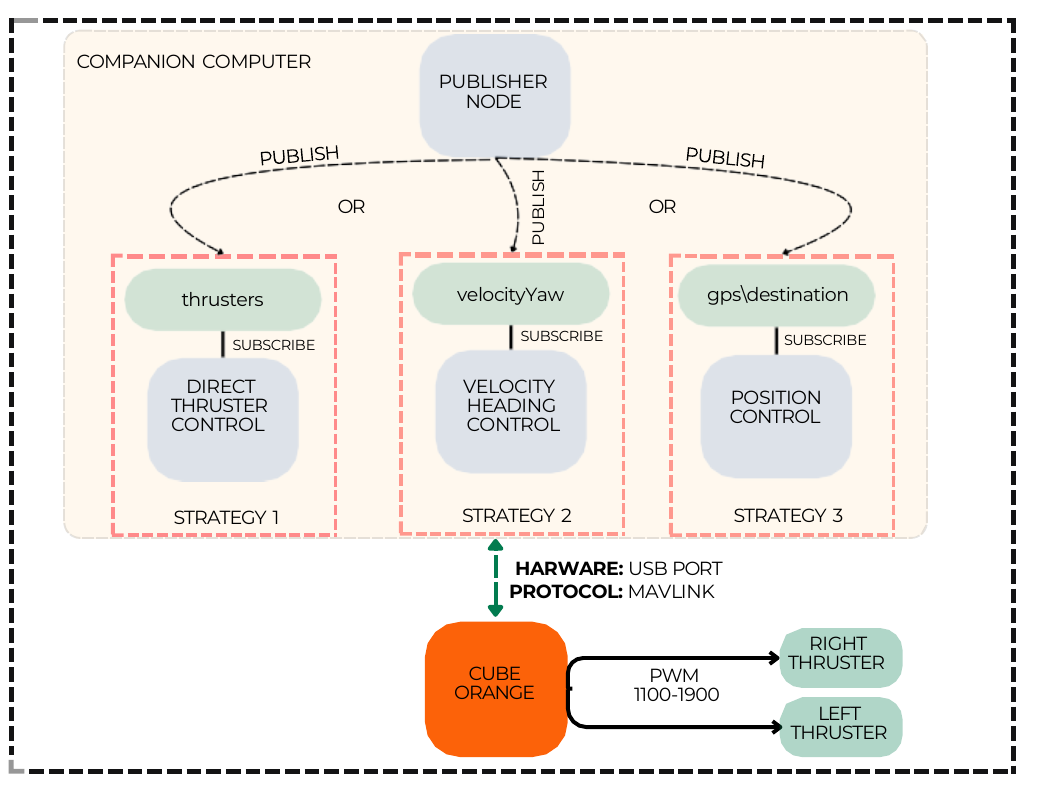
\includegraphics[width=0.8\textwidth]{fig/fig_ros2_mavlink_kumar2025.png}
  \caption{Uso de nodos de ROS~2 y del protocolo MAVLink para el control de un USV ~\cite{kumar2025}.}
  \label{fig:ros2_mavlink}
\end{figure}

\FloatBarrier
 
El ecosistema de ROS~2 incluye, además, herramientas de apoyo al desarrollo: rosbag2
graba los mensajes de los tópicos seleccionados, con su marca de tiempo, para analizarlos
y reproducirlos una vez finalizada la misión~\cite{sears2024} \cite{Cite18}, y el simulador
Gazebo permite depurar algoritmos sobre un modelo virtual del vehículo antes de su
despliegue~\cite{aliane2026}.
 
% =====================================================================
% Sección 2.5 Comunicaciones inalámbricas y mecanismos de recuperación
% Requiere: amsmath
% =====================================================================
 
\section{Comunicaciones inalámbricas y mecanismos de recuperación}
\label{sec:comunicaciones}
 
% ---------------------------------------------------------------------
\subsection{Topologías y enlaces inalámbricos}
\label{subsec:topologias}
 
La comunicación entre varios vehículos no tripulados y su estación de control puede
organizarse en tres topologías~\cite{Cite26}. En la topología punto a punto (P2P), cada
vehículo se enlaza directamente con la estación. En la topología punto a multipunto
(P2M), o en estrella, todos los vehículos se conectan a un nodo central que retransmite
la información, de modo que la comunicación entre dos vehículos atraviesa dos enlaces.
En la topología en malla, los vehículos intercambian datos entre sí y los reenvían hacia
la estación, a costa de una mayor complejidad de encaminamiento~\cite{Cite26}.
 
La elección de un enlace inalámbrico está condicionada por su banda de frecuencia, que
determina un compromiso entre alcance y capacidad. Las bandas por debajo de 1\,GHz
sufren menores pérdidas de propagación y toleran mejor los obstáculos, lo que permite
alcances de decenas de kilómetros con potencias del orden de 1\,W, pero sus canales
estrechos limitan la tasa de datos a cientos de kbit/s. Por ello, los radiomódems de
estas bandas se emplean como enlaces serie transparentes para la telemetría y el mando
del autopiloto~\cite{gogendeau2024} \cite{Cite10}. Las bandas superiores, como la de 5\,GHz,
admiten canales más anchos y, con ello, una capacidad muy superior, suficiente para
transmitir imágenes y datos de mayor volumen, pero su alcance depende en mayor medida de
mantener una línea de vista despejada entre las antenas. Estos sistemas suelen operar
como redes locales en estrella, en las que un punto de acceso en la estación base da
servicio a varias estaciones, una en cada vehículo~\cite{Cite25}. Por estas
características complementarias, en vehículos de superficie de bajo coste es habitual
combinar ambos tipos de enlace~\cite{gogendeau2024}. En todos los casos, el alcance
real queda limitado por la altura de las antenas sobre el agua y por los obstáculos del
entorno, y suele ser bastante inferior al nominal, como muestran los alcances de entre
0,5 y 1\,km reportados en campo para enlaces WiFi~\cite{sears2024}.
 
La coexistencia de ambos enlaces aporta redundancia: al operar en bandas de frecuencia y
con tecnologías distintas, la pérdida de uno de ellos no implica la pérdida total de
supervisión y control del vehículo~\cite{Cite26}.
 
% ---------------------------------------------------------------------
\subsection{Métricas de desempeño de un enlace}
\label{subsec:metricas_enlace}
 
El desempeño de un enlace de comunicación se caracteriza principalmente mediante su
latencia y su pérdida de paquetes~\cite{Cite26}, junto con la variación de la latencia. La latencia es el
tiempo que tarda un mensaje en llegar de un extremo al otro. Medirla de forma directa
exige que los relojes de emisor y receptor estén sincronizados, por lo que en la práctica
se mide el tiempo de ida y vuelta (RTT), es decir, el tiempo que transcurre desde que
se envía un mensaje hasta que se recibe su respuesta, por ejemplo mediante mensajes de
eco ICMP~\cite{Cite26}. Suponiendo que el trayecto de ida y el de vuelta son simétricos,
la latencia en un sentido se estima como
\begin{equation}
  d_{k} \approx \frac{\mathrm{RTT}_{k}}{2}
  \label{eq:latencia_rtt}
\end{equation}
donde $\mathrm{RTT}_{k}$ es el tiempo de ida y vuelta del mensaje $k$. En una topología
en estrella, la latencia entre dos vehículos es aproximadamente la suma de las
latencias de cada vehículo con el nodo central.
 
La variación de la latencia entre mensajes consecutivos, conocida como \textit{jitter},
indica la regularidad con que llegan los datos y puede estimarse como el valor medio de
las diferencias sucesivas de latencia:
\begin{equation}
  J = \frac{1}{N-1}\sum_{k=1}^{N-1}\left| d_{k+1} - d_{k} \right|
  \label{eq:jitter}
\end{equation}
Por último, la tasa de pérdida de paquetes expresa la proporción de mensajes enviados
que no llegan a su destino:
\begin{equation}
  P_{\mathrm{p}} = \frac{N_{\mathrm{env}} - N_{\mathrm{rec}}}{N_{\mathrm{env}}}\cdot 100\,\%
  \label{eq:perdida_paquetes}
\end{equation}
donde $N_{\mathrm{env}}$ y $N_{\mathrm{rec}}$ son el número de mensajes enviados y
recibidos. Estas tres magnitudes se degradan a medida que aumenta la distancia o se
obstruye la línea de vista, por lo que el alcance efectivo de un enlace se define, en la
práctica, como la distancia a partir de la cual dejan de cumplirse los valores
admisibles.
 
% ---------------------------------------------------------------------
\subsection{Mecanismos de recuperación ante fallos}
\label{subsec:failsafe}
 
Los autopilotos incorporan mecanismos de seguridad (\textit{failsafe}) que ejecutan una
acción automática cuando detectan una condición anómala, como una batería baja, un
fallo de la misión~\cite{kumar2025} o una pérdida de calidad de la estimación de
posición, que el autopiloto supervisa de forma continua a partir de las lecturas del
receptor GNSS~\cite{kumar2025} \cite{aliane2026}.
La acción más habitual es el retorno autónomo al punto de partida mediante el modo
\textit{RTL}, descrito en la Sección~\ref{subsec:mavros}, aunque también puede optarse
por mantener la posición del vehículo mediante el modo \textit{Loiter}~\cite{kumar2025}. Estos mecanismos pueden
complementarse desde el ordenador a bordo, que supervisa condiciones adicionales, como
la velocidad del viento o el estado de la batería, y envía al autopiloto la orden de
retorno; en campo se han medido retardos medios de unos 5\,s entre la detección de la
condición de riesgo y la activación del retorno~\cite{sotelo2023}. A todo ello se suma la
recuperación manual: mediante un conmutador de la emisora de radiocontrol, el operador
puede devolver el vehículo al modo \textit{Manual} y retomar su control directo en
cualquier momento~\cite{iniesta2025}.